\documentclass[nobib]{tufte-handout}

\title{Lecture 6: Weights, distances, and minimum spanning trees $\cdot$ 1MA020}

\author[Vilhelm Agdur]{Vilhelm Agdur\thanks{\href{mailto:vilhelm.agdur@math.uu.se}{\nolinkurl{vilhelm.agdur@math.uu.se}}}}

\date{13 November 2023}


%\geometry{showframe} % display margins for debugging page layout

\usepackage{graphicx} % allow embedded images
  \setkeys{Gin}{width=\linewidth,totalheight=\textheight,keepaspectratio}
  \graphicspath{{graphics/}} % set of paths to search for images
\usepackage{amsmath}  % extended mathematics
\usepackage{booktabs} % book-quality tables
\usepackage{units}    % non-stacked fractions and better unit spacing
\usepackage{multicol} % multiple column layout facilities
\usepackage{lipsum}   % filler text
\usepackage{fancyvrb} % extended verbatim environments
  \fvset{fontsize=\normalsize}% default font size for fancy-verbatim environments

\usepackage{color,soul} % Highlights for text

% Standardize command font styles and environments
\newcommand{\doccmd}[1]{\texttt{\textbackslash#1}}% command name -- adds backslash automatically
\newcommand{\docopt}[1]{\ensuremath{\langle}\textrm{\textit{#1}}\ensuremath{\rangle}}% optional command argument
\newcommand{\docarg}[1]{\textrm{\textit{#1}}}% (required) command argument
\newcommand{\docenv}[1]{\textsf{#1}}% environment name
\newcommand{\docpkg}[1]{\texttt{#1}}% package name
\newcommand{\doccls}[1]{\texttt{#1}}% document class name
\newcommand{\docclsopt}[1]{\texttt{#1}}% document class option name
\newenvironment{docspec}{\begin{quote}\noindent}{\end{quote}}% command specification environment

\include{mathcommands.extratex}

\begin{document}

\maketitle% this prints the handout title, author, and date

\begin{abstract}
\noindent
Continuing from our previous discussion on the existence of spanning trees and counting of them, we come to the problem of actually finding them. We give two different algorithms for this. Finally we consider the problem of computing distances in a graph, and give an algorithm for this.
\end{abstract}

As we saw in the exercises in our previous session, the question of spanning trees becomes more interesting if we also add weights to the edges of our graph, since we can then consider the \emph{minimum} spanning trees.

We also saw that to do this, we need to restrict ourselves to finite graphs,\sidenote[][]{Later, when we measure distances, we will also need to assume all weights are positive, or we will again have silly things happen.} or stupid things will happen. If we additionally assume that all weights are distinct, there is even a \emph{unique} minimal spanning tree.

\section{Prim's algorithm}

The first algorithm we introduce for this is Prim's algorithm, which works by starting in a particular vertex and growing the tree.

\begin{figure}
  \centering
  \includegraphics[width=0.85\textwidth]{graphics/L6_prim_kruskal_dijkstra/prims_algorithm.png}
  \caption[][0cm]{An illustration of how Prim's algorithm finds a minimal spanning tree in a graph.}
  \label{fig:prims_algorithm}
\end{figure}

\begin{definition}[Prim's algorithm]
  Let $G = (V,E,w)$ be a finite connected weighted graph, and let $v \in V$ be an arbitrary vertex of $G$.
\begin{enumerate}
    \item Initialise a tree $T = (\{v\}, \emptyset)$, i.e. the subtree containing only $v$.
    \item While $T$ is not a spanning subgraph, i.e. $V(T) \neq V$, find an edge $e$ of $G$ between $V(T)$ and $V(T)^c$ (all vertices in $G$ that are not in $T$) which has minimal weight. Add this edge together with its endpoint in $V(T)^c$ to $T$.
    \item Return $T$.
    \end{enumerate}
  How this algorithm constructs an MST is illustrated in Figure \ref{fig:prims_algorithm}.
\end{definition}

Before we can prove that this algorithm actually works, we will need a little lemma about what happens when you remove edges from trees.\sidenote[][]{This statement is perhaps in some sense obvious, but it did not occur to me immediately. The proof in the old lecture notes omits the steps that would even require the lemma, and the proofs I found online did not omit those steps but did leave the lemma implicit.}

\begin{lemma} \label{lemma:removing_edges_from_trees}
  If $T = (V, E)$ is a tree and $e = (u, w)$ an edge of $T$, then $F = (V, E \setminus e)$, the graph gotten by removing the edge $e$ from $T$, has exactly two connected components, both of which are trees.

  More generally, removing $k$ edges from a tree will create $k+1$ connected components, each of which is a tree.
  
  \begin{proof}
    That the connected components of a graph gotten by removing edges from a tree will always be trees is easy to see -- they are by definition connected, and removing edges can't have introduced any cycles, so they are connected and acyclic, i.e. trees.\sidenote[][]{A graph all of whose connected components are trees is called a \emph{forest}, of course. These are precisely the acyclic graphs. So one very poor definition of ``tree'' could be ``a tree is a connected forest''.}

    Now, to see that $F$ must have exactly two connected components, let $U$ be the connected component containing $u$, and $W$ be the connected component containing $w$. Assume $v$ is some vertex not in $U$ -- we will show it is then in $W$.

    Since $T$ is connected, there is a path $P$ connecting $v$ to $u$ -- and since $v$ is not in $U$, this path must have been destroyed by removing the edge $e$. Now, since $e = (w, u)$ is incident to $u$, it must in fact have been the final edge of the path $P$, so we can write
    $$P = v\, e_1\, v_1\, e_2\, \ldots\, e_\ell\, w\, e\, u.$$
    
    This however means that by removing the last edge of $P$ we get a path from $v$ to $w$, proving that $v \in W$, as desired.

    The result for a general number of edges removed follows by induction from the one-edge case.
  \end{proof}
\end{lemma}

\begin{theorem}
  Prim's algorithm is correct, that is, it always generates a minimum spanning tree.

  \begin{proof}
    Let $G = (V,E,w)$ be a finite connected weighted graph, and let the sequence of subgraphs that Prim's algorithm creates be $T_0 \subseteq T_1 \subseteq \ldots \subseteq T_{n-1} = T$. It is easy to see that $T_i$ will always be connected and have $i$ edges, so $T_{n-1}$ has to be a tree, so Prim's algorithm at least always finds \emph{a} spanning tree.
    
    To see that this spanning tree is minimal, we consider an MST $T'$, and show that $w(T) \leq w(T')$. If $T = T'$ we are done, so assume they are distinct, and let
    $$j = \max\left\{i \in \{0,1,\ldots,n-1\} \given T_i \subseteq T'\right\}.$$
    That is, $j$ is the final time at which all edges of $T_j$ are also edges of $T'$.

    So, let $e = (u, w)$ be the edge between $V(T_j)$ and $V(T_j)^c$ added by the next step of the algorithm, with $u \in V(T_j)$ and $w \in V(T_j)^c$. By assumption, this edge is not in $T'$.
    
    Since $T'$ is a tree, there must be a unique path in $T'$ connecting $u$ and $w$, and at some point this path must cross from $V(T_j)$ into $V(T_j)^c$. Call the edge it crosses with $f = (u', w')$.

    By construction, $e$ has minimal weight among all edges between $V(T_j)$ and $V(T_j)^c$, so we must have $w(e) \leq w(f)$. Let us now show that we can modify the tree $T'$ into a different spanning tree $T''$ which contains $e$ and satisfies $w(T'') \leq w(T')$, so that $T''$ is also an MST.

    The way we do this is of course by removing the edge $f$ from $T'$ and adding the edge $e$. It is clear that this does not increase the weight of the graph, so the thing we need to show is that it is still a tree. 
    
    It follows from Lemma \ref{lemma:removing_edges_from_trees} that removing the edge $f$ yields a graph with two connected components, $V(T_j)$ and $V(T_j)^c$, each of which is a tree. Clearly the edge $e$ also goes between these components, so adding it back in will reconnect the two trees, and that adding an edge between two disconnected trees yields a tree is clear, since it connects the graph and can't possibly add a cycle.

    So we can repeat this process inductively, taking the new tree $T''$ as the new MST with which we compare $T$, until eventually $T = T^{'''\cdots'''}$ and so $T$ is an MST.
  \end{proof}
\end{theorem}

\begin{remark}
  The runtime of this algorithm will depend on the implementation -- specifically on how the graph is represented\sidenote[][-0.9cm]{Are you storing essentially an adjacency matrix, or a list of edges, or something like a ``linked list'' kind of structure? There are many ways of representing a graph in memory.} and on how you find the next edge between $V(T_i)$ and $V(T_i)^c$. A good implementation has a runtime of $O\left(\abs{E} + \abs{V}\log\left(\abs{V}\right)\right)$.\sidenote[][]{If you just store an adjacency matrix, you get a runtime of $O\left(\abs{V}^2\right)$, while if you store the graph as a list of vertices, where each vertex is a list of its neighbours, and use a Fibonacci heap to help finding the minimal edges, you get the runtime of the ``good'' implementation.}
\end{remark}

\section{Kruskal's algorithm}

The second algorithm we consider for finding MSTs is \emph{Kruskal's algorithm}, which doesn't iteratively create larger trees, but instead creates a forest that grows until it becomes a tree.

\begin{figure}
  \centering
  \includegraphics[width=0.85\textwidth]{graphics/L6_prim_kruskal_dijkstra/kruskals_algorithm.png}
  \caption[][0cm]{An illustration of how Kruskal's algorithm finds a minimal spanning tree in the same graph as the one in Figure \ref{fig:prims_algorithm}, which illustrated Prim's algorithm.}
  \label{fig:kruskals_algorithm}
\end{figure}

\begin{definition}[Kruskal's algorithm]
  Let $G = (V,E,w)$ be a connected finite weighted graph, and let $L$ be a list of the edges of $G$ sorted in ascending order of weight.
  \begin{enumerate}
      \item Initialise the forest $F = (V, \emptyset)$. 
      \item While $F$ is not spanning remove the first entry from $L$, and call it $e$. If adding $e$ to $F$ would not create a cycle add $e$ to $F$.
      \item Return $F$.
    \end{enumerate}
  How this algorithm constructs an MST is illustrated in Figure \ref{fig:kruskals_algorithm}.
\end{definition}

\begin{theorem}
  Kruskal's algorithm is correct, that is, it always generates an MST.

  \begin{proof}
    Let $G = (V,E,w)$ be a finite connected weighted graph. It is clear by construction that Kruskal's algorithm always generates a cycle-free spanning subgraph which is edge maximal, and so by a similar argument as when we were proving all graphs have spanning trees, it must always generate a spanning tree.

    To see that this spanning tree is in fact maximal, we again compare with a known MST. In particular, let $T$ be the spanning tree found by Kruskal's algorithm, and let $T'$ denote an MST that has a maximal number of edges shared with $T$. We will show that if $T \neq T'$ we can actually modify $T'$ to have even more edges in common with $T$, while still being an MST, contradicting our maximality assumption, and so we must have $T = T'$.

    So, assuming $T \neq T'$, let $e$ be the lowest-weight edge of $T$ that is not contained in $T'$. Adding $e$ to $T'$ will create a cycle, and somewhere on this cycle there must be an edge $f$ not contained in $T$.

    Our modification of $T'$ will be to remove $f$ and add $e$, getting a new spanning tree $T''$.\sidenote[][]{
      \begin{xca}
        Prove that $T''$ actually is a spanning tree.
      \end{xca}
    } Since $T'$ is an MST, $w(T') \leq w(T'')$. On the other hand, since Kruskal's algorithm chose to add $e$ instead of $f$ when given the choice, we must have $w(e) \leq w(f)$, and so therefore we also have $w(T'') \leq w(T')$, and so $w(T') = w(T'')$, and $T''$ is also an MST. This, however, gives us our contradiction, since $T''$ shares more edges with $T$ than $T'$ did.
  \end{proof}
\end{theorem}

\begin{remark}
  Kruskal's algorithm has a runtime of $O\left(\abs{E}\log\left(\abs{V}\right)\right)$, but if you are already given the edges sorted by weight, it runs in $O\left(\abs{E}\mathop{\alpha}\left(\abs{V}\right)\right)$ time, where $\alpha$ is the inverse of the Ackermann function.
\end{remark}

\section{Graph distances}

Another thing we did in our exercises was to consider distance functions on graphs. Recall the following definition from the exercises:

\begin{definition}
  For a weighted graph $G$ with positive edge-weights, we define the \emph{graph distance} between two vertices $v, v' \in G$ by
  $$d_G(v, v') = \min_{\text{walks }P\text{ from }v\text{ to }v'} \sum_{e \in E(P)} w(e).$$
\end{definition}

We proved during the exercises that this actually is a metric on the set of vertices whenever the graph is connected, so it makes sense to call this a distance and use the language of metric spaces. We can also extend this definition to disconnected metric spaces if we recall the convention that a minimum over an empty set is $\infty$.\sidenote[][]{This is really the same thing as why an empty sum is zero, an empty product $1$, an empty union is $\emptyset$, and so on.}

\begin{definition}
  The \emph{diameter} of a graph is the same as the diameter for any metric space -- it is the maximum distance between any two vertices.\sidenote[][]{This has also been called ``longest shortest path'', presumably by people who like confusing terminology.} That is,
  $$\diam(G) = \max_{v, u \in V(G)} d(v,u).$$
\end{definition}

Instead of trying to compute the diameter of a graph, let us just try to compute the distance between two vertices. Or rather, it turns out to not be markedly harder to compute the distance between a given vertex and every other vertex, so we give an algorithm that can do this, and then we will say how to turn this into an algorithm for the simpler problem.

In fact, we can interpret the problem of finding the distances between a given vertex and the rest of the graph as a problem of finding a certain spanning tree, rooted at the given vertex. If we just let each vertex pick its neighbour closest to the root as its parent, tiebreaking arbitrarily\sidenote[][]{That is, if a vertex has two neighbours that minimize the distance to the root, we pick one of them arbitrarily.}, this tree precisely encodes the information we need.\sidenote[][]{
  \begin{xca}
    Prove that this really is a tree. You can equivalently think of it as the union of all shortest paths between the root $v$ and some other vertex. (This tree is called a shortest-path tree.)
  \end{xca}
}

\begin{figure}
  \centering
  \includegraphics[width=0.85\textwidth]{graphics/L6_prim_kruskal_dijkstra/dijkstras_algorithm.png}
  \caption[][0cm]{An illustration of how Dijkstra's algorithm finds a shortest path tree in a graph. Edge weights are given in blue, the distance function $d(v_0, \cdot)$ is given in red, and the parent function $p$ is indicated by the red arrows pointing along edges.}
  \label{fig:dijkstras_algorithm}
\end{figure}

\begin{definition}[Dijkstra's algorithm]
  We take as arguments a weighted graph $G = (V,E,w)$ and an initial vertex $v_0$, and the state of the algorithm consists of a \emph{currently visited vertex} $v$, a set $Q$ of \emph{unvisited vertices}, a partially function $p: V \to V$ assigning each vertex its \emph{parent}, and a \emph{distance function} $d(v_0, \cdot)$. 
  
  We initialize the algorithm by setting $v = v_0$, $Q = V$, $p(v_0) = v_0$ and undefined otherwise, and
  $$d(v_0, v) = \begin{cases}
    0&\text{if }v=v_0\\
    \infty&\text{otherwise.}
  \end{cases}$$

  In each time step, we do the following:
  \begin{enumerate}
    \item Remove the currently visited vertex $v$ from $Q$.
    \item For each neighbour $v'$ of $v$, check whether
          $$d(v_0, v) + w(\{v, v'\}) < d(v_0, v').$$
          If this is the case, going from $v'$ to $v$ and then back to $v_0$ gives a shorter path to $v_0$ than previously known, so we set $d(v_0, v')$ to $d(v_0, v) + w(\{v, v'\})$ and let $p(v')$ be $v$.
    \item If $Q$ contains a vertex with finite value of $d(v_0, \cdot)$,\sidenote[][]{The reason we phrase it like this is that we want the algorithm to be able to handle disconnected graphs as well. If $G$ is disconnected, $Q$ will never be empty, but the things in different connected components will have distance $\infty$ even after we have seen the entire connected component of $v_0$.} we set the new currently visited vertex to be the vertex $v$ in $Q$ with smallest $d(v_0,v)$. Otherwise, the algorithm terminates and returns the distance function $d$ and the parent function $p$.
  \end{enumerate}

  How this algorithm works is illustrated in Figure \ref{fig:dijkstras_algorithm}.
\end{definition}

\begin{remark}
  If we are only interested in the distance to some specific vertex $v'$, we can find the distance to it by terminating the algorithm already when $v'$ is the currently visited vertex.

  If we want to find the actual path that realizes the found distance, we can just iterate the parent function $p$ -- starting in a vertex $v$, walk to $p(v)$, then to $p(p(v))$, and so on until you reach $v_0$.

  With the right implementation, Dijkstra's algorithm has a runtime of $O\left(\abs{E} + \abs{V}\log\left(\abs{V}\right)\right)$.
\end{remark}

\section{Exercises}
 
\begin{xca}
  We have shown in an exercise during our previous exercise session\sidenote[][]{If you did not solve that exercise, a proof is also in last years lecture notes.} that a weighted graph with all weights distinct has a unique minimum spanning tree.

  Is the stronger statement that in fact no two spanning trees have the same weight also true?
\end{xca}

\begin{xca}
  One way to find a path between two vertices is to first find a minimum spanning tree for the graph and then find the unique path between them in this tree. Will this always be the shortest path between them?

  If not, will there always be \emph{some} pair of vertices such that this is the shortest path between them?
\end{xca}

\begin{xca}
  Are any of the things we did in this lecture useful for computing the diameter of a graph? Think about how one might do it, and what runtimes your suggested algorithms will have.\sidenote[][]{You can then, if you like, spend some time googling to learn what the best approaches known achieve.}
\end{xca}

\begin{xca}
Use Prim's algorithm and Kruskal's algorithm to find the minimum spanning tree of the graph in figure \ref{fig:new_exercise}.
\begin{figure}
    \centering
    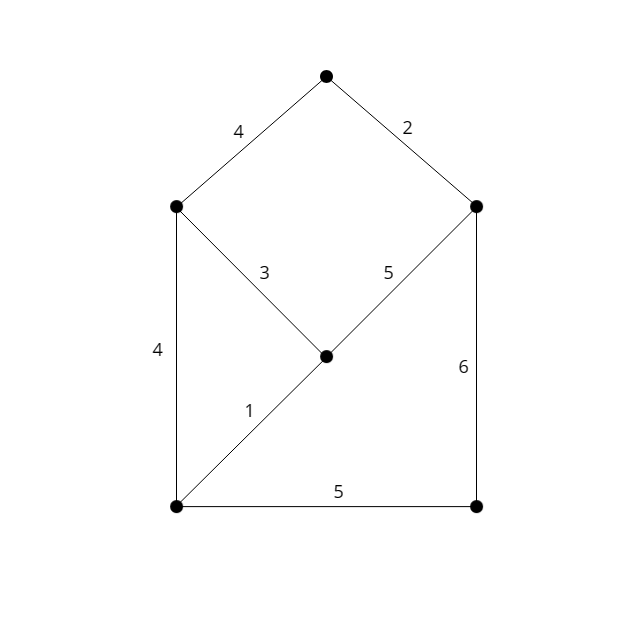
\includegraphics[width=0.7\textwidth]{graphics/L6_prim_kruskal_dijkstra/graph_exc6-7.png}
    \caption{Graph for exercise 6 and 7.}
    \label{fig:new_exercise}
\end{figure}
\end{xca}

\begin{xca}
Implement Dijkstras algorithm on the graph in Figure \ref{fig:new_exercise} using the vertex in the lower left corner as the initial vertex $v_0$.
\end{xca}


%\bibliography{references}
%\bibliographystyle{plainnat}

\end{document}
